%% Template file for all Software/Hardware modules

\subsection{Add-Ons}
The Server provides for the computational needs of the POW-R project; 
More hardware shall be added before the utility needs of the project are met.

\subsubsection{IP Display}
The IP of the Server shall be displayed somewhere on it's casing. 
The user will enter this IP into their browser to access the Display.

This will be achieved by connecting an Arduino via USB to the Server, and housing it inside the Server's casing. 
The Arduino will be connected to an LCD display which will output the network IP of the Server. 
Figure \ref{ArduinoLCD} shows the interaction between Server and Arduino.

\begin{figure}
\centering
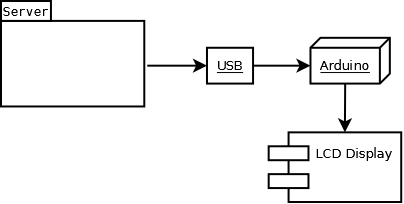
\includegraphics[scale=0.5]{Hardware/images/ArduinoLCD.png}
\caption{IP Display Diagram}
\label{ArduinoLCD}
\end{figure}

The IP of the system can be obtained via kernel module, and sent to the Arduino one byte at a time. 
This works well, since the Arduino connects over serial and thusly takes a byte at a time.

\subsection{GPIO Pins}
As mentioned above in the "PC Hardware" section, the mainboard is outfitted with a GPIO pin header. 
A Linux distribution will be used for the Server's operating system, which must support interaction with such pins. 

A folder can be found in the Linux kernel, at the location \filename{/sys/class/gpio} that helps with GPIO manipulation. 
To set up a single GPIO pin, one must type the following command into a terminal (as root):

\begin{lstlisting}
	$ echo N > /sys/class/gpio/export
	(where N must be a GPIO pin number)
\end{lstlisting}

When this command is issued, a directory is made inside the \filename{gpio} directory, named \filename{gpioN}, where N is the GPIO pin number you passed. 
Two files will be in that new directory, \filename{direction} and \filename{value}. 
\filename{direction} can only contain "in" or "out" with no leading characters, spaces, line breaks, etc.
\filename{value} can only contain "1" or "0" and can be read or written to at any time.
These files, \filename{direction} and \filename{value} are responsible for what kind of pin it is (input or output) and what the current value is (1 or 0), respectively.

NOTE: The pin number you must echo into \filename{/sys/class/gpio/export} is not necessarily the number of the actual pin on the board, but may refer to the pin of the bridge that connects the GPIO port to the motherboard.

The subsections below are buttons that the Server must have, and each of these buttons connects to a GPIO pin.


\subsubsection{Power Switch}
A standard rocker switch will be added to the case to provide the user with a way to turn the Server on and off. 
The style of the switch will clearly signify "On" or "Off".

\subsubsection{Factory Reset*}
This button should intentionally be placed somewhere inconvenient: 
Sunken into the case far enough that you need a skinny rod (such as a paperclip) to push it, and in a spot
that chaotic forces (children, mean people, God's divine will) will not notice it.

\subsubsection{Connect to Satellite}
A button will be added to the Server that allows a user to add a Satellite easily.
When a user wants to add a Satellite to the network, the following series of events should take place, in order:

\begin{itemize}
	\item User plugs Satellite into wall outlet
	\item User presses "connect" button on Satellite
	\item User presses "connect" button on Server
	\item Satellite is now connected
\end{itemize}
	
\subsection{Server Hull}
The Server needs a protective casing, for several reasons. 
On the physical level, a durable casing will protect the hardware. 
The casing also serves to render unnecessary ports inaccessible to users. 
Lastly, the casing is important in the sense that the term "Server" currently only applies to the mainboard, 
and most people think of a legitimate Server as something physical, encased in a box, that's protected and hidden away, exactly as a Server should be.

As far as prototyping goes, the casing can be as simple as a folded piece of aluminum
with holes cut in it to fit the IP display, the buttons, and any ports that must be
exposed. As an end-game product, the casing would probably be a little less "junkyard."
